\section{Background and Motivation}

\subsection{Coded Distributed Learning}

In synchronous distributed learning, the training data are split into
$m$ shards and the master coordinates one gradient computation at iteration
$t$.  Let $w_t$ be the current model and let $g_j(w_t)$ denote the partial
gradient computed from shard $j$.  The full gradient is
\begin{equation}
  \label{eq:full-gradient}
  g(w_t) = \sum_{j=1}^{m} g_j(w_t),
\end{equation}
so an uncoded synchronous system must wait until every shard contribution has
arrived.  Gradient coding~\cite{tandon2017gradient} and related coded
computation methods~\cite{lee2018speeding} avoid this all-worker wait by
asking workers to compute encoded linear combinations of shard gradients.  The
master then reconstructs the same vector $g(w_t)$ after receiving a sufficient
subset of encoded results.

\subsection{Sparse Flexible Coded Computing}

Sparse flexible coded learning constructs a code matrix by stacking two sparse
row blocks
\begin{equation}
  \label{eq:sfcl-code}
  B =
  \begin{bmatrix}
    A^{(1)} \\
    A^{(2)}
\end{bmatrix}
  \in \mathbb{R}^{2n \times m},
\end{equation}
where $n$ is the number of workers and $m$ is the number of data shards.  The
matrix in Equation~\eqref{eq:sfcl-code} has one column per shard and $2n$
encoded rows.  Let $b_r^\top$ be row $r$ of $B$; the coefficient $b_{rj}$ says
how shard $j$ participates in encoded row $r$.  A zero coefficient means that
row $r$ does not touch shard $j$, which is where sparsity reduces arithmetic
work.  Let
$G_t=[g_1(w_t),\ldots,g_m(w_t)]^\top$ denote the stack of shard gradients at
iteration $t$.  Encoded row $r$ computes the vector
\begin{equation}
  \label{eq:encoded-row}
  \tilde{g}_r = b_r^\top G_t = \sum_{j=1}^{m} b_{rj} g_j(w_t).
\end{equation}
Equation~\eqref{eq:encoded-row} uses $b_r^\top G_t$ as shorthand for the
weighted vector sum on the right-hand side.  Let
$S \subseteq \{1,\ldots,2n\}$ be the indexes of encoded rows that have
completed and returned to the master.  Define
$B_S \in \mathbb{R}^{|S|\times m}$ as the submatrix of $B$ formed by selecting
the completed rows in $S$.  The master can decode once
\begin{equation}
  \label{eq:decode-span}
  \mathbf{1}_m \in \mathrm{span}(B_S^\top).
\end{equation}
Here $\mathbf{1}_m$ is the all-ones vector of length $m$, because recovering the
full gradient in Equation~\eqref{eq:full-gradient} requires coefficient one on
every shard gradient.
The notation $\mathrm{span}(B_S^\top)$ denotes the column span of
$B_S^\top$, equivalently all linear combinations of the completed row
coefficient vectors.  Thus Equation~\eqref{eq:decode-span} says that the
completed rows can be linearly combined to produce the all-ones coefficient
vector.  Equivalently, there exists a decoding vector
$c_S \in \mathbb{R}^{|S|}$ such that
\begin{equation}
  \label{eq:decode-vector}
  B_S^\top c_S = \mathbf{1}_m.
\end{equation}
Multiplying the received encoded gradients by the same coefficients $c_S$
recovers the uncoded full gradient $g(w_t)$.

Decodability is decoder-dependent.  Equations~\eqref{eq:decode-span}
and~\eqref{eq:decode-vector} describe exact linear decoding, as implemented by
a rank or Gaussian-elimination-style solve.  A peeling or BP decoder would use a
different success predicate based on whether iterative singleton recovery can
finish.  Such a predicate can be stricter than the span condition: a returned
row set may be linearly sufficient for Gaussian decoding but not peelable by
BP.  This paper uses the exact row-span predicate throughout; BP-aware
first-decodable scheduling is a natural extension with a different decoder
predicate.

The sparse flexible construction mainly decides which rows exist and how sparse
they are.  In a cloud system, the runtime must also decide which row pair goes
to which worker.  This paper focuses on that runtime degree of freedom.

\subsection{Cost-Only Assignment Failure}
\label{sec:motivation}

Sparse encoded rows have different arithmetic costs because they touch
different numbers of nonzero data blocks.  A cost-aware scheduler assigns
expensive rows to fast workers.  This can reduce total completed computation
time, but the first decodable set may depend on rows that are not locally most
expensive.  If such rows are delayed, the master still waits even though many
other rows have finished.

Figure~\ref{fig:motivation} illustrates this gap with one iteration of a fixed
code.  The code already makes the pair $\{r_2,r_5\}$ a legal recovery set.  A
cost-aware order sorts work by local row cost and worker speed, without asking
which rows jointly make the target decodable; in the example, it exposes
$r_3$ and $r_6$ before both recovery rows have arrived.  A decode-aware order
instead tries to expose a legal recovery set early; here, it places $r_2$ and
$r_5$ in the first two completions.  The runtime gap is therefore the
difference between the first decodable times, not a difference in code
construction.  The guard enables adaptive placement only when the predicted
prefix reduction is large enough to dominate scheduling, extra-work,
communication, and cancellation costs.

\begin{figure}[t]
  \centering
  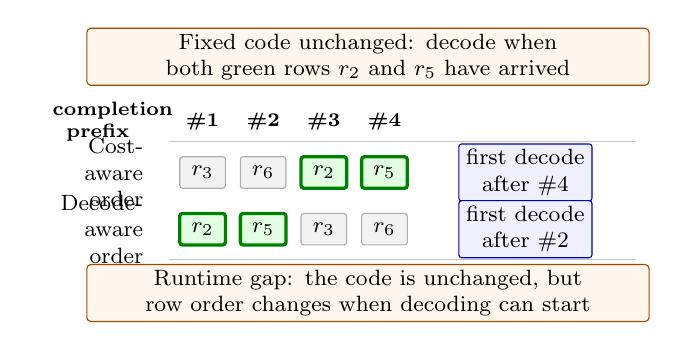
\begin{tikzpicture}[
      font=\footnotesize,
      row/.style={draw, rounded corners=1pt, align=center,
        minimum width=0.58cm, minimum height=0.40cm, inner sep=1pt},
      crit/.style={row, fill=green!11, draw=green!50!black, very thick},
      other/.style={row, fill=gray!10, draw=gray!65},
      marker/.style={draw=blue!70!black, fill=blue!6, rounded corners=1pt,
        align=center, inner sep=2pt, text width=1.55cm},
      note/.style={draw, rounded corners=1.5pt, align=center, inner sep=2pt,
        fill=orange!7, draw=orange!60!black},
      head/.style={font=\scriptsize\bfseries, align=center},
      sep/.style={gray!45, line width=0.25pt}
    ]
    \node[note, text width=7.0cm] at (3.45,0)
      {Fixed code unchanged: decode when both green rows $r_2$ and $r_5$ have arrived};

    \node[head, anchor=east, text width=1.15cm] at (0.72,-0.82) {completion\\prefix};
    \node[head] at (1.35,-0.82) {\#1};
    \node[head] at (2.12,-0.82) {\#2};
    \node[head] at (2.89,-0.82) {\#3};
    \node[head] at (3.66,-0.82) {\#4};
    \draw[sep] (0.92,-1.07) -- (6.85,-1.07);

    \node[anchor=east, align=right, text width=1.35cm] at (0.72,-1.47)
      {Cost-aware\\order};
    \node[other] (c1) at (1.35,-1.47) {$r_3$};
    \node[other] (c2) at (2.12,-1.47) {$r_6$};
    \node[crit]  (c3) at (2.89,-1.47) {$r_2$};
    \node[crit]  (c4) at (3.66,-1.47) {$r_5$};
    \node[marker] (cd) at (5.45,-1.47) {first decode\\after \#4};

    \node[anchor=east, align=right, text width=1.35cm] at (0.72,-2.19)
      {Decode-aware\\order};
    \node[crit]  (f1) at (1.35,-2.19) {$r_2$};
    \node[crit]  (f2) at (2.12,-2.19) {$r_5$};
    \node[other] (f3) at (2.89,-2.19) {$r_3$};
    \node[other] (f4) at (3.66,-2.19) {$r_6$};
    \node[marker] (fd) at (5.45,-2.19) {first decode\\after \#2};

    \draw[sep] (0.92,-2.57) -- (6.85,-2.57);
    \node[note, text width=7.0cm] at (3.45,-3.00)
      {Runtime gap: the code is unchanged, but row order changes when decoding can start};
  \end{tikzpicture}
  \caption{Row completion order changes the first-decodable prefix even when
  the code is fixed.}
  \Description{A timeline-style example. The same fixed code allows rows r2
  and r5 to decode. Under cost-aware order, two other rows finish first and
  decoding happens at prefix four. Under decode-aware order, r2 and r5
  finish first and decoding happens at prefix two.}
  \label{fig:motivation}
\end{figure}

We verify the effect in Figure~\ref{fig:motivation} with a deliberately small
mechanism diagnostic before introducing the design.  The diagnostic fixes an
8-worker/8-shard sparse-flexible code, generates five code instances, samples
12 worker-state rounds per instance, and changes only the row-pair priority
used to expose rows.  For each round, it predicts row completion times from
sparse row costs and sampled worker speeds, then runs the same row-span check
after each completion to find the first-decodable prefix.  Static placement has
31.6 ms predicted mean first-decode time.  A cost-only priority improves the
mean to 25.4 ms, but still needs 9.1 completed rows on average before decode.
An oracle decode-priority order, computed by enumerating minimal decodable
subsets in this tiny code, reaches 19.3 ms and reduces the first-decodable
prefix by 1.2 rows relative to static placement.  The oracle is not a deployable
scheduler, and the diagnostic does not include network or service overhead; it
isolates the reason Figure~\ref{fig:motivation} matters.  The design below
therefore uses cheap decodability-aware row scores and an online guard rather
than treating row cost alone as the scheduling objective.
